\documentclass[
  coursetitle={Cómputo Nube y Tecnologías Emergentes},
  coursehours={96},
  coursedate={Verano 2026},
  doctype={Notas de clase},
  otherlangs={english,french},
  authorname={Lázaro},
  authorsurname={Bustio-Martínez},
  authortitle={PhD},
  role={Profesor Investigador},
  email={lbustio@inaoe.mx},
  phone={5559504000},
  ext={7459},
  institution={Instituto Nacional de Astrofísica, Óptica y Electrónica (INAOE)},
  department={Maestría en Ciencias en Tecnologías de Seguridad},
  address={Luis Enrique Erro 1, Sta. Ma. Tonantzintla, San Andrés Cholula, CP 72840, Puebla, México},
  margin={0.5in}
]{../../lbustio_lecture_notes}

\usepackage[utf8]{inputenc}
\usepackage[T1]{fontenc}
\usepackage{array}
\usepackage{tabularx}
\usepackage{enumitem}
\usepackage{longtable}
\usepackage{booktabs}
\usepackage{url}
\usepackage{listings}
\usepackage{xcolor}
\usepackage{graphicx}
\usepackage{tcolorbox}
\usepackage{amsmath}
\usepackage{tikz}
\usetikzlibrary{arrows.meta,backgrounds,fit,positioning,shapes.geometric}

\definecolor{lightgray}{rgb}{0.97, 0.97, 0.97}
\definecolor{darkblue}{rgb}{0, 0, 0.6}
\definecolor{gcpblue}{HTML}{4285F4}
\definecolor{gcpgreen}{HTML}{34A853}
\definecolor{gcpyellow}{HTML}{FBBC04}
\definecolor{gcpred}{HTML}{EA4335}
\definecolor{softgray}{HTML}{F5F7FA}
\definecolor{chainblue}{HTML}{1A56DB}
\definecolor{chaindark}{HTML}{0D2B6E}
\definecolor{chaingreen}{HTML}{057A55}
\definecolor{chainred}{HTML}{C81E1E}
\definecolor{chaingray}{HTML}{6B7280}

\lstset{
  backgroundcolor=\color{lightgray},
  basicstyle=\ttfamily\small,
  breaklines=true,
  frame=single,
  columns=fullflexible,
  showstringspaces=false,
  commentstyle=\color{chaingray},
  keywordstyle=\color{darkblue},
  inputencoding=utf8,
  extendedchars=true,
  literate={á}{{\'a}}1 {é}{{\'e}}1 {í}{{\'i}}1 {ó}{{\'o}}1 {ú}{{\'u}}1 {ñ}{{\~n}}1
           {Á}{{\'A}}1 {É}{{\'E}}1 {Í}{{\'I}}1 {Ó}{{\'O}}1 {Ú}{{\'U}}1 {Ñ}{{\~N}}1
}

\setlist[itemize]{topsep=0.3em,itemsep=0.2em}
\setlist[enumerate]{topsep=0.3em,itemsep=0.2em}

\tikzset{
  block/.style={
    draw=chaindark,
    fill=chainblue!10,
    rounded corners=4pt,
    very thick,
    align=left,
    text width=3.6cm,
    minimum height=3.2cm,
    inner sep=8pt,
    font=\small
  },
  genesisblock/.style={
    block,
    draw=chaingreen,
    fill=chaingreen!10
  },
  chainlink/.style={
    -{Latex[length=3.5mm,width=2.5mm]},
    very thick,
    draw=chaindark
  },
  hashbox/.style={
    draw=gcpred,
    fill=gcpred!8,
    rounded corners=3pt,
    thick,
    align=center,
    font=\ttfamily\scriptsize,
    inner sep=4pt
  },
  concept/.style={
    draw=chainblue,
    fill=chainblue!7,
    rounded corners=4pt,
    thick,
    align=center,
    text width=2.5cm,
    minimum height=1.1cm,
    inner sep=5pt,
    font=\small
  },
  flowarrow/.style={
    -{Latex[length=3mm,width=2mm]},
    thick,
    draw=chaindark
  }
}

\begin{document}

\IberoCover

\section{¿Qué es blockchain?}

Blockchain es una estructura de datos distribuida que registra información en bloques enlazados mediante funciones hash criptográficas. Una vez que un bloque es añadido a la cadena, modificar su contenido invalida todos los bloques siguientes, lo que hace que la manipulación sea detectable.

\begin{tcolorbox}[title=Concepto central]
Blockchain NO es sinónimo de criptomoneda. Es un mecanismo para \textbf{registrar, validar, proteger y verificar información} de forma distribuida y resistente a la manipulación. Las criptomonedas son una de sus aplicaciones, pero no la única.
\end{tcolorbox}

Las propiedades fundamentales que distinguen a una blockchain de una base de datos convencional son:

\begin{description}
  \item[Inmutabilidad.] Los registros almacenados no pueden modificarse retroactivamente sin invalidar la cadena completa.
  \item[Descentralización.] No existe una autoridad central que controle la cadena; múltiples nodos mantienen copias idénticas.
  \item[Transparencia.] Cualquier participante puede auditar el historial completo de transacciones.
  \item[Resistencia a la censura.] No hay un punto único de fallo ni de control.
  \item[Trazabilidad.] Cada transacción queda registrada con un identificador único y un sello temporal.
\end{description}

\section{Estructura de un bloque}

Un bloque es la unidad de almacenamiento básica de una blockchain. Cada bloque contiene un encabezado con metadatos y un cuerpo con las transacciones o datos registrados.

\subsection{Campos del encabezado}

\begin{description}
  \item[Índice (\texttt{index}).] Número de posición del bloque en la cadena. El primer bloque tiene índice 0.
  \item[Sello temporal (\texttt{timestamp}).] Momento en que el bloque fue creado o minado.
  \item[Hash del bloque (\texttt{hash}).] Huella digital del bloque, calculada aplicando una función hash sobre todos sus campos.
  \item[Hash del bloque anterior (\texttt{previous\_hash}).] El hash del bloque inmediatamente anterior. Este campo es el mecanismo de enlace de la cadena.
  \item[Nonce.] Número arbitrario que se ajusta durante el proceso de minería para satisfacer la condición de dificultad del proof of work.
  \item[Datos / transacciones.] El contenido efectivo registrado en el bloque.
\end{description}

\subsection{Representación de la cadena}

El siguiente diagrama muestra una cadena de tres bloques. El bloque génesis tiene como hash anterior una cadena de ceros, convención que indica el inicio de la cadena.

\begin{center}
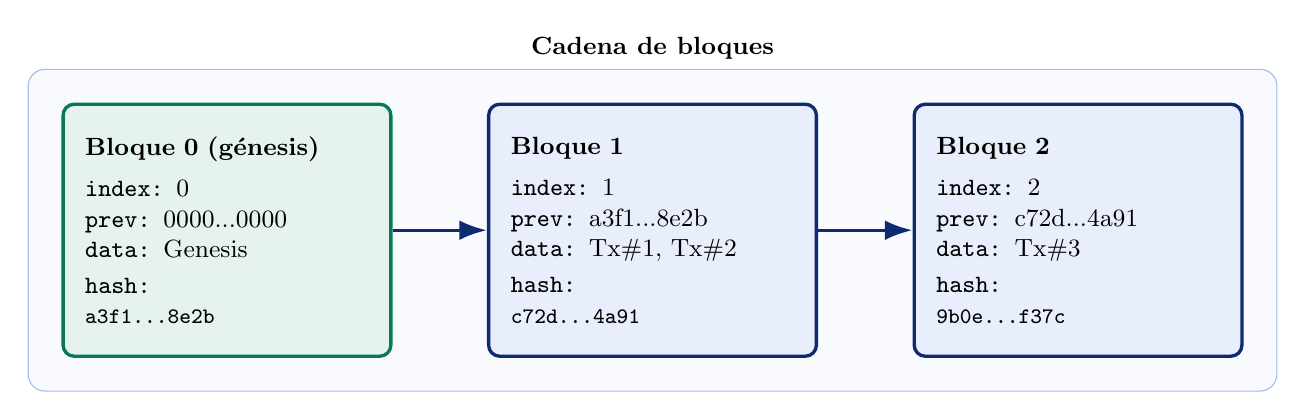
\begin{tikzpicture}[node distance=0.7cm]

  \node[genesisblock] (b0) {
    \textbf{Bloque 0 (génesis)}\\[4pt]
    \texttt{index:} 0\\
    \texttt{prev:} 0000...0000\\
    \texttt{data:} Genesis\\[2pt]
    \texttt{hash:}\\
    \texttt{\footnotesize a3f1...8e2b}
  };

  \node[block, right=1.2cm of b0] (b1) {
    \textbf{Bloque 1}\\[4pt]
    \texttt{index:} 1\\
    \texttt{prev:} a3f1...8e2b\\
    \texttt{data:} Tx\#1, Tx\#2\\[2pt]
    \texttt{hash:}\\
    \texttt{\footnotesize c72d...4a91}
  };

  \node[block, right=1.2cm of b1] (b2) {
    \textbf{Bloque 2}\\[4pt]
    \texttt{index:} 2\\
    \texttt{prev:} c72d...4a91\\
    \texttt{data:} Tx\#3\\[2pt]
    \texttt{hash:}\\
    \texttt{\footnotesize 9b0e...f37c}
  };

  \draw[chainlink] (b0.east) -- (b1.west);
  \draw[chainlink] (b1.east) -- (b2.west);

  \begin{scope}[on background layer]
    \node[
      draw=chainblue!40,
      fill=chainblue!3,
      rounded corners=6pt,
      inner sep=12pt,
      fit=(b0)(b1)(b2),
      label={[font=\bfseries\small]above:Cadena de bloques}
    ] {};
  \end{scope}
\end{tikzpicture}

\small\textbf{Figura:} Tres bloques enlazados mediante el campo \texttt{previous\_hash}.
\end{center}

\section{Funciones hash criptográficas}

Una función hash es el mecanismo que garantiza la integridad de la cadena. Toma una entrada de longitud arbitraria y produce una salida de longitud fija (el hash o huella digital), con las siguientes propiedades:

\begin{enumerate}
  \item \textbf{Determinismo:} la misma entrada siempre produce el mismo hash.
  \item \textbf{Velocidad:} el cálculo es computacionalmente eficiente.
  \item \textbf{Efecto avalancha:} un cambio mínimo en la entrada produce un hash completamente diferente.
  \item \textbf{Resistencia a preimagen:} dado un hash, es computacionalmente inviable encontrar la entrada original.
  \item \textbf{Resistencia a colisiones:} es computacionalmente inviable encontrar dos entradas distintas con el mismo hash.
\end{enumerate}

\begin{tcolorbox}[title=Por qué el hash garantiza la integridad]
Si alguien modifica el contenido del bloque 1, su hash cambia. El bloque 2 almacena el hash anterior del bloque 1, por lo que ahora el bloque 2 queda invalidado. Para ``reparar'' la cadena, habría que recalcular todos los bloques desde el bloque 1 en adelante --- y hacerlo más rápido que el resto de la red. En una red suficientemente grande, esto es computacionalmente inviable.
\end{tcolorbox}

La blockchain educativa utilizada en este curso calcula el hash de cada bloque con SHA-256 sobre la concatenación de sus campos:

\begin{lstlisting}
hash = SHA256(index + timestamp + previous_hash + data + nonce)
\end{lstlisting}

\section{Transacciones}

Una transacción es la unidad mínima de información que se registra en la blockchain. Dependiendo de la aplicación, una transacción puede representar:

\begin{itemize}
  \item una transferencia de valor entre dos partes (criptomonedas);
  \item el hash de un archivo para verificar su integridad;
  \item un evento de seguridad (inicio de sesión, acceso a recurso, alerta);
  \item un registro de auditoría firmado digitalmente;
  \item un contrato o acuerdo entre partes.
\end{itemize}

En la blockchain educativa de este curso, las transacciones son objetos JSON con estructura libre. El nodo registra las transacciones pendientes en un pool y las incluye en el siguiente bloque durante el proceso de minería.

\subsection{Ciclo de vida de una transacción}

\begin{center}
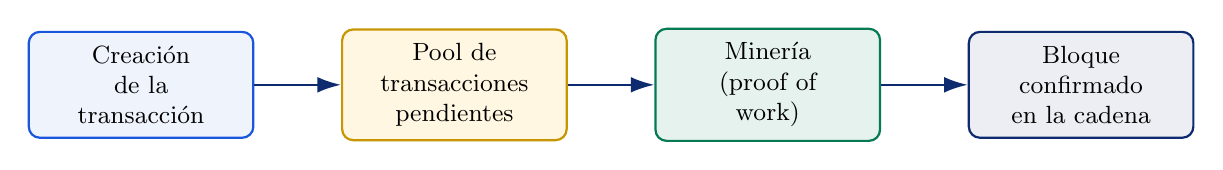
\begin{tikzpicture}[node distance=0.5cm and 1.1cm]
  \node[concept, draw=chainblue] (creation) {Creación\\de la\\transacción};
  \node[concept, draw=gcpyellow!80!black, fill=gcpyellow!12, right=of creation] (pool) {Pool de\\transacciones\\pendientes};
  \node[concept, draw=chaingreen, fill=chaingreen!10, right=of pool] (mining) {Minería\\(proof of\\work)};
  \node[concept, draw=chaindark, fill=chaindark!8, right=of mining] (block) {Bloque\\confirmado\\en la cadena};

  \draw[flowarrow] (creation) -- (pool);
  \draw[flowarrow] (pool) -- (mining);
  \draw[flowarrow] (mining) -- (block);
\end{tikzpicture}

\small\textbf{Figura:} Ciclo de vida de una transacción desde su creación hasta su confirmación.
\end{center}

\section{Mecanismos de consenso}

El consenso es el proceso mediante el cual los nodos de una red descentralizada se ponen de acuerdo sobre el estado válido de la cadena. Distintas blockchains utilizan distintos mecanismos de consenso.

\subsection{Proof of Work (PoW)}

Es el mecanismo original de Bitcoin. Los nodos (mineros) compiten por encontrar un \textit{nonce} tal que el hash del bloque comience con un número mínimo de ceros (la \textit{dificultad}):

\begin{lstlisting}
while not hash(block).startswith("0" * difficulty):
    block.nonce += 1
\end{lstlisting}

El primer nodo en encontrar el nonce válido difunde el bloque a la red y recibe una recompensa. La dificultad se ajusta para que la generación de bloques ocurra a una tasa constante.

\textbf{Ventajas:} simple, probado, resistente a ataques Sybil.\\
\textbf{Desventajas:} alto consumo energético, baja escalabilidad.

\subsection{Proof of Stake (PoS)}

Los validadores son seleccionados en proporción a la cantidad de tokens que han bloqueado como garantía (\textit{stake}). Si actúan deshonestamente, pierden su garantía.

\textbf{Ventajas:} menor consumo energético, mayor escalabilidad.\\
\textbf{Desventajas:} puede favorecer a los más ricos, complejidad de diseño.

\subsection{Consenso simplificado en la blockchain educativa}

La blockchain educativa de este curso implementa un proof of work simplificado con dificultad configurable. Su objetivo no es seguridad de red sino demostrar el principio de la minería y la generación de bloques de forma observable y reproducible.

\section{Arquitectura de una red blockchain}

\begin{center}
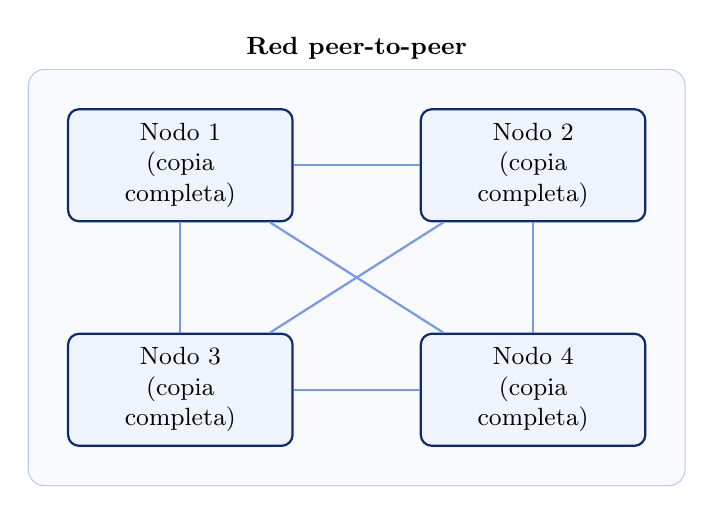
\begin{tikzpicture}[node distance=1.4cm and 1.6cm]
  \node[concept, draw=chaindark] (n1) {Nodo 1\\(copia\\completa)};
  \node[concept, draw=chaindark, right=of n1] (n2) {Nodo 2\\(copia\\completa)};
  \node[concept, draw=chaindark, below=of n1] (n3) {Nodo 3\\(copia\\completa)};
  \node[concept, draw=chaindark, right=of n3] (n4) {Nodo 4\\(copia\\completa)};

  \draw[thick, draw=chainblue!60] (n1) -- (n2);
  \draw[thick, draw=chainblue!60] (n1) -- (n3);
  \draw[thick, draw=chainblue!60] (n1) -- (n4);
  \draw[thick, draw=chainblue!60] (n2) -- (n4);
  \draw[thick, draw=chainblue!60] (n3) -- (n4);
  \draw[thick, draw=chainblue!60] (n2) -- (n3);

  \begin{scope}[on background layer]
    \node[
      draw=chainblue!30,
      fill=chainblue!3,
      rounded corners=6pt,
      inner sep=14pt,
      fit=(n1)(n2)(n3)(n4),
      label={[font=\bfseries\small]above:Red peer-to-peer}
    ] {};
  \end{scope}
\end{tikzpicture}

\small\textbf{Figura:} Cada nodo mantiene una copia completa e idéntica de la cadena. No existe servidor central.
\end{center}

\section{APIs blockchain}

En la práctica de este curso la blockchain expone una API REST que permite interactuar con la cadena mediante peticiones HTTP. Los endpoints principales son:

\begin{center}
\begin{tabular}{lll}
\hline
\textbf{Método} & \textbf{Endpoint} & \textbf{Descripción} \\
\hline
\texttt{GET}  & \texttt{/chain}              & Devuelve la cadena completa \\
\texttt{GET}  & \texttt{/blocks/<index>}      & Devuelve un bloque por índice \\
\texttt{GET}  & \texttt{/validate}            & Valida la integridad de la cadena \\
\texttt{POST} & \texttt{/transactions/new}    & Crea una nueva transacción pendiente \\
\texttt{POST} & \texttt{/mine}                & Mina un nuevo bloque \\
\hline
\end{tabular}
\end{center}

La interacción con la API se realiza mediante \texttt{curl} o cualquier cliente HTTP. El formato de intercambio es JSON.

\section{Blockchain y ciberseguridad}

Blockchain ofrece propiedades que son directamente aplicables a problemas de seguridad. A continuación se presentan los casos de uso más relevantes en el contexto del curso.

\subsection{Integridad de registros}

Los logs de seguridad pueden ser manipulados por un atacante que haya comprometido el sistema. Almacenar el hash de cada entrada de log en una blockchain hace que la alteración sea detectable: modificar el log cambiaría su hash, que ya no coincidiría con el registrado en la cadena.

\subsection{Trazabilidad y auditoría}

La inmutabilidad de la cadena convierte a blockchain en un registro de auditoría confiable. Cada transacción queda asociada a un sello temporal y no puede borrarse ni modificarse retroactivamente.

\subsection{Verificación de evidencia digital}

En investigaciones forenses, es fundamental demostrar que la evidencia no fue alterada desde su recolección. Registrar el hash de la evidencia en una blockchain en el momento de su captura proporciona una prueba criptográfica de integridad.

\subsection{Registro de eventos de seguridad}

Accesos, autenticaciones, cambios de configuración y alertas pueden registrarse en una blockchain privada, creando un historial inmutable y auditable de actividad del sistema.

\begin{tcolorbox}[title=Limitación importante]
Blockchain garantiza la integridad de los datos \textbf{después} de ser registrados. No garantiza que los datos registrados sean verídicos; eso depende de la fuente. Un log incorrecto registrado en la blockchain seguirá siendo incorrecto, pero no podrá ser modificado sin detección.
\end{tcolorbox}

\section{Criptomonedas y contratos inteligentes}

\subsection{Bitcoin}

Bitcoin fue la primera aplicación masiva de blockchain, propuesta por Satoshi Nakamoto en 2008. Es una moneda digital descentralizada que permite transferencias entre partes sin necesidad de intermediarios financieros. Sus bloques almacenan exclusivamente transacciones de valor.

\subsection{Ethereum}

Ethereum extendió el modelo de Bitcoin con la capacidad de ejecutar \textit{contratos inteligentes}: programas almacenados en la blockchain que se ejecutan automáticamente cuando se cumplen las condiciones especificadas en su código.

\subsection{Contratos inteligentes}

Un contrato inteligente (smart contract) es un programa que reside en la blockchain y cuya ejecución es determinista, transparente y no puede ser detenida ni alterada una vez desplegado. Permite automatizar acuerdos sin necesidad de un intermediario de confianza.

Aplicaciones en ciberseguridad:
\begin{itemize}
  \item gestión automática de identidades y permisos;
  \item liberación condicional de credenciales de acceso;
  \item pagos automáticos vinculados a la entrega verificada de servicios;
  \item registro inmutable de acuerdos entre organizaciones.
\end{itemize}

\subsection{Stablecoins y tokenización}

Las \textit{stablecoins} son criptomonedas cuyo valor está vinculado a un activo estable (generalmente el dólar estadounidense) para evitar la volatilidad típica de Bitcoin y Ethereum.

La \textit{tokenización} es la representación digital de activos del mundo real (inmuebles, acciones, obras de arte, identidades, documentos) como tokens en una blockchain. Permite fraccionar, transferir y auditar la propiedad de activos de forma programable.

\section{Limitaciones y riesgos de blockchain}

Blockchain no es una solución universal. Es importante evaluar críticamente sus limitaciones antes de considerarla para un caso de uso específico.

\begin{description}
  \item[Escalabilidad.] Las blockchains públicas tienen capacidad de procesamiento de transacciones muy limitada en comparación con sistemas centralizados. Bitcoin procesa aproximadamente 7 transacciones por segundo; Visa procesa miles.
  \item[Consumo energético.] El proof of work requiere grandes cantidades de energía para la minería. Es una de las principales críticas medioambientales de las blockchains públicas.
  \item[Latencia.] La confirmación de una transacción puede tardar minutos u horas, dependiendo de la red y el mecanismo de consenso.
  \item[Privacidad.] La transparencia de la cadena puede ser indeseable en ciertos contextos. Aunque los participantes se identifican por claves públicas, el análisis de transacciones puede revelar patrones de comportamiento.
  \item[Irreversibilidad.] Un error en una transacción no puede corregirse; solo puede compensarse con una nueva transacción. Esto introduce riesgos operativos importantes.
  \item[Gobernanza.] En redes descentralizadas, tomar decisiones colectivas sobre cambios al protocolo es un proceso lento y conflictivo.
  \item[Complejidad de desarrollo.] Los contratos inteligentes son difíciles de auditar y depurar. Errores en su código pueden ser explotados irreversiblemente.
  \item[Centralización práctica.] En la práctica, grandes pools de minería y proveedores de infraestructura concentran el poder de red, contradiciendo el principio de descentralización.
\end{description}

\begin{tcolorbox}[title=Cuándo blockchain tiene sentido]
Blockchain es adecuada cuando se requiere un registro compartido entre partes que \textbf{no se confían mutuamente}, sin necesidad de un intermediario central, con requisitos de inmutabilidad y auditoría. Si existe un administrador central de confianza, una base de datos convencional es más eficiente, más barata y más fácil de mantener.
\end{tcolorbox}

\section{Comparación: blockchain vs. base de datos convencional}

\begin{center}
\begin{tabular}{lcc}
\hline
\textbf{Característica} & \textbf{Blockchain} & \textbf{Base de datos} \\
\hline
Control centralizado       & No         & Sí \\
Inmutabilidad              & Sí         & No (por diseño) \\
Transparencia              & Alta       & Configurable \\
Velocidad de escritura     & Baja       & Alta \\
Escalabilidad              & Limitada   & Alta \\
Costo operativo            & Alto       & Bajo \\
Modificación de registros  & Detectable & Posible \\
Requiere consenso          & Sí         & No \\
\hline
\end{tabular}
\end{center}

\section{La práctica del módulo}

En las próximas sesiones desplegaremos e interactuaremos con una blockchain educativa ligera implementada en Python y Flask sobre una máquina virtual en Google Cloud Platform.

La blockchain educativa implementa:
\begin{itemize}
  \item estructura real de bloques con hash SHA-256;
  \item enlace de bloques mediante \texttt{previous\_hash};
  \item pool de transacciones pendientes;
  \item proof of work simplificado con dificultad configurable;
  \item validación de integridad de la cadena completa;
  \item API REST para interacción externa mediante \texttt{curl}.
\end{itemize}

El objetivo de la práctica no es replicar una blockchain de producción, sino comprender y verificar experimentalmente los principios que la hacen funcionar.

\begin{tcolorbox}[title=Prerequisito para la próxima sesión]
Para la sesión práctica del 29 de junio, el estudiante debe tener disponible una VM Linux en GCP con acceso SSH y los puertos necesarios abiertos en las reglas de firewall. Se reutilizará la infraestructura desplegada en módulos anteriores.
\end{tcolorbox}

\end{document}
